
\documentclass[a4paper,12pt,twoside]{memoir}

%inkluderte pakker

\usepackage[utf8]{inputenc}
\usepackage{hyperref}
\usepackage{paralist}
\usepackage{graphicx}
\usepackage{cite}


%slutt på pakkene


\begin{document}

%%Her begynner oversettelsen til norsk
			\renewcommand{\chaptername}{Del}
            \renewcommand{\contentsname}{Innhold}
            \renewcommand\listfigurename{Illustrasjoner}
            \renewcommand\tablename{Tabell}
			\renewcommand\listtablename{Tabeller}
            \renewcommand{\figurename}{Illustrasjon}

%%Her slutter den

\frontmatter
%Grafisk Forside

	\newcommand\nbvspace[1][3]{\vspace*{\stretch{#1}}}
	% allow some slack to avoid under/overfull boxes
	\newcommand\nbstretchyspace{\spaceskip0.5em plus 0.25em minus 0.25em}
	% To improve spacing on titlepages
	\newcommand{\nbtitlestretch}{\spaceskip0.6em}
	\pagestyle{empty}
	\begin{center}
	\bfseries
	\nbvspace[1]
	\Huge
	{\nbtitlestretch\huge
	Forelesningsmateriale\\ Fagakademiet}

	\nbvspace[1]
	\normalsize

	Kliniske problemstillinger i hjemmetjenesten\\
	med pasienteksempler\\
	\nbvspace[1]
	\small av\\
	\Large Pål Ager- Wick\\[0.5em]
	\footnotesize Kommuneoverlege\\

	\nbvspace[2]

	%\includegraphics[width=6in]{./anitascotland.jpg} %placeholder for ete bilde på forsiden
	\nbvspace[3]
	\normalsize

	Tønsberg\\
	\large
	01.12.2013\\
	\nbvspace[1]
	\end{center}

%Slutt grafisk forside

		\chapter{Forord}%!!!
				Denne boken er et vedlegg til fagdagen i arrangert av fagakademiet. Målgruppen en er helsepersonell med utdannelse som helsefagarbeider eller sykepleier. Det vil kanskje være noe av informasjonen som er litt kort presentert eller til og med ufullstendig. Det er fordi at vi forutsetter forkunnskaper. Bakerst finnes referanser og litteraturanbefalinger for de som er interessert.
				\\[0.7in]



				DRAMMEN 26.10.2013\\[0.4in]

				Pål CJ Ager-Wick

	\newpage
	\tableofcontents

\mainmatter
	\chapter{Hvordan jobbe systematisk}
		\section{Å lage verktøy for å ikke være redd}
			\paragraph{Hvorfor blir vi engstelige?\\}
				Det er utfordrende å jobbe i fremste rekke. Risikoen kan være høy. Men hva skjer dersom noe går galt. Mange av mottakerne av hjemmetjenester er eldre eller har flere sykdommer. Det kan være vanskelig kjenne igjen symptomer på alvorlige sykdommer, men også hva de forskjellige trenger. Noen ganger skjer ting som gjør helsepersonellet usikre eller redde.
			\paragraph{Glemsk?\\}
				Det er alltid mye nytt om behandling av kjente sykdommer. Det kan være veldig mye å sette seg inn i. Den menneskelige hjerne kan huske 7-9 ting på en gang. Det kan være utfordrende huske på alt sammen. Men samtidig kan vi som helsepersonell mye om sykdommer. Huskelister kan være en måte å redusere komplikasjoner på\cite{FA-gawande}.
		\section{Lær av feil}
			\paragraph{Endel av hverdagen vår\\}
				Å være helsepersonell vil gjøre at man må håndtere feil. Det er ingen som ønsker å gjøre feil, men det hender likevel alle. Når det skjer er det desto viktigere å lære av dem.
			\paragraph{I system\\}
				For å unngå å gjennta feil eller avdekke dem på systemnivå, må vi ha et system for å fange dem opp. Avviksmeldinger kan være kjedelig ekstraarbeid som kommer på toppen av alt i en travel hverdag. Likevel er det bare slik man kan lære.
		\section{Hvordan finne god informasjon}
			\paragraph{Jeg lurer på...\\}
				Hvor slår du opp hvis du lurer på noe. Det er ikke sikkert at alle internettkilder er like pålitelige. Hvem svarer på alle spørmålene som dukker opp i løpet av en travel arbeiddag. Det er veldig viktig å ha system på dette for å sørge for at all informasjonen vi bruker er kvalitetssikret. 
			\paragraph{Hvem bestemmer hvordan pasienter skal behandles?\\}
				Det finnes mange veiledere fra helsedirektoratet som gir retningslinjer. Andre ressurser er \href{http://www.helsebiblioteket.no/}{helsebiblioteket.no}. Det viktigste er at alle i tjenesten engasjeres i å utvikle faget, og at man får tid til det. 
		%\section{Sjekklister fra bakken og opp?}
		%\section{Systemer er kjedelig} Beholde?
		%\section{Noen praktiske prinsipper}
	\chapter{Hjertesykdommer}
		\chapterprecishere{Vuuuu, vuu vuu\par\raggedleft--- \textup{Molly}, En husky hund fra Drammen}
		Her er noen få av alle hjertesykdommene forklart. Dette er ment å være et tillegg til forelesningen slik at man ikke må notere så mye. Dette er ikke en fullstendig oversikt over hjertesykdommene. Det er også forsøkt å forklare på et så enkelt som mulig nivå slik at hjertespesialister eller andre vil føle at det er litt enkelt. Dette materialet er ikke laget for dem.\\
		\section{Anatomi}
			\paragraph{Slik ser hjerte ut\\}
					\begin{figure}[ht]
                      \centering
                      	\frame{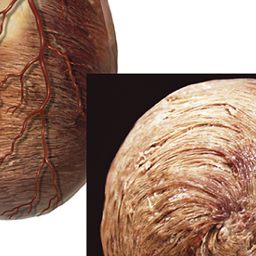
\includegraphics[width=5in]{./kap/bilder/hjerte}}%!!! må byttes ut, copyright saladin
                      \caption{Et hjerte}
                      {Her ser vi et hjerte som er fiksert i formalin.}%\textit{tjenestetilbudene}.]
                    \end{figure}    


				%!!! Her må et bilde inn
			\paragraph{Effektiv jobbing\\}
				Når hjertet pumper med vanlig frekvens er det veldig effektivt. Da sørger det for jevn transport av blodet på en mest mulig energieffektiv måte. Når hjerteslagene blir veldig raske blir hjertet mindre effektivt\cite{FA-saladin}. Man kan kalle det en funksjonell hjertesvikt. Det betyr at hjertet er friskt, men jobber på- eller over grensen for at blodet skal strømme fritt.
				%legg inn video an ultralyd ecco cor!!!
		\section{Fysiologi}	
			\paragraph{Hva menes med hjerte- og karsykdommer?\\}\label{sec:athero}
				Som alle organer i kroppen har hjertet sine egne blodårer. De er ekstra utsatt for åreforkalking, eller atherosklerose som det heter på latin. Atherosklerose er kalkinnlagring i blodåreveggen som gjør den stiv og samtidig klumpete på innsiden. Dette hindrer blodgjennomstrømningen. Mengden med kalk i blodårene er varierende gjennom livet, men fet mat, høyt blodtrykk og sigaretter gjør at mer kalk lagres. 
		\section{Patologi}	
			\paragraph{Skader oppstår\\}
				Noen steder blir blodpassasjen dårlig og det kan dannes skader fordi vevet ikke får nok oksygen. Hjertet er en muskel med innebygget nervesystem og noen ganger blir det små skader som gror til arr i forkammeret. Dette kan skape atrieflimmer\cite{!!!}. Hvis blodårene tetter seg rundt hjertekammeret får man ofte anginasmerter, og dersom blodåren blir helt tett er det et infarkt.
		\section{Klinikk}
			\subsection{Hjerteinfarkt}	
				\paragraph{Symptomer\\}
					Trykkende smerte i brystet, utstråling til venstre arm eller underkjeve. Blek og kaldsvett, klam og tungpusten. Dette er noen klassiske symptomer ved hjerteinfarkt. Vi må passe oss fordi, eldre, pasienter med diabetes eller kvinner har ofte helt andre symptomer. 
				\paragraph{Førstehjelp\\}
					Ring ambulansen, vær hos pasienten. Gi oksygen og Dispiril hvis dere har. 
				\paragraph{Farlige momenter\\}
					De som dør av hjerteinfarkt får ofte akutt hjertflimmer. Dette er ikke atriflimmer, men kammerflimmer og er helt forskjellig. Hjertet slår med 300 slag i minuttet. Pasienten er bevisstløs og den eneste redningen er å bruke hjertestarter og å gjøre hjerte- lungeredning. Det viktigste for akutte hjerteinfarkt er rask behandling med utblokking og innsetting av stent. Noen pasienter egner seg ikke for dette, særlig de eldste og sykeste ville ikke overleve behandlingen og blir heller behandlet på sykehus uten utblokking. 
				\paragraph{Hva skjer etterpå?\\}
					Alle pasienter som har hatt hjerteinfarkt får nesten samme type medisiner:
					\begin{itemize}
						\item Metoprolol(SelZok(R)), gjør at hjertet for "hvile". Forebygger nye infarkt og hjerterytmeforstyrrelser. Senker blodtrykket, og gjør at makspulsen blir lavere ved fysiske anstrengelser. Noen menn blir impotente. Kalles også "Betablokker"\\
						\item Acetylsalisylsyre\\%!!!
					\end{itemize}
				\paragraph{Tips for hverdagen\\}
					Hjertesyke pasienter bør man passe på brå endringer i tilstanden, dette gjelder forøvrig alle andre sykdomstilstander som blir beskrevet her. Hvis en pasient har kjent hjertesykdom og lav "blodprosent" kan den lave blodprosenten utløse infarkt.
			\subsection{Hjertesvikt}
				Er oftest en komplikasjon etter et hjerteinfarkt som ikke ble behandlet i tide. New York Heart Assosiation(NYHA) har klassifisert hjertesvikt etter hvordan pasientene fungere i hverdagen. 
				% NYHA -bilde!!!
				%
				\paragraph{Symtomer\\}
					Tungpust og hovne bein. Slapphet og trettbarhet. Dårlig matlyst.
				\paragraph{Hva må helsepersonell passe på\\}
					Følg med på vekten. En hjertesviktpasient kan gå opp i vekt med flere kilo om dagen dersom medisinene slutter å fungere. 
				\paragraph{Hvor farlig er det\\}
					Jo høyere grad hjertesvikt jo dødligere er det. En alvorlig hjertesvikt er å sammenligne med kreftsykdommer med spredning. Ikke glem å rådføre med lindrende avdeling når det gjelder disse pasientene.
				\paragraph{Tips for hverdagen\\}
					Ikke glem å veie hjertesviktpasienter. Alle med hejrtesvikt bør føre drikkeskjema fordi for mye drikke kan forverre symptomene. 
			\subsection{Atrieflimmer}
				Noen ganger utvikler hjertet en feil i det elektriske systemet. Dette fører til atrieflimmer, som ofte kommer anfallsvis. Når blodet utsettes for ujevne hjerteslag kan det klumpe seg og føre til hjerneslag.
				\paragraph{Symptomer\\}
					Samme som hjertesvikt, men kommer ganske akutt. Pulsen er ujevn og rask. 
				\paragraph{Hva må hjemmetjenesten være oppmerksomme på?\\}
					Å drikke lite gjør at pasientene kan få anfall. Hvis blodfortynningen ikke er tilstrekkelig, vil pasientene kunne få slag. Derfor er det viktig å følge med på INR. 
				\paragraph{Medisiner\\}
					Metoprolol begrenser hjerterytmen og forebygger anfall. Marevan forebygger hjerneslag. Noen nye behandlinger er under innføring for eksempel Rivaroxiban(Xarelto(r)), som også virker blodfortynnende. Noen pasienter får Digitalis(Digoxin(r), Digitoxin(r)), som det står mer om i neste kapittel.
			\subsection{Digitalis}
				Digitalis er et naturprodukt som er veldig giftig. Det styrker hjertemuskelens evne til å slå og stabiliserer hjerterytmen.
				\paragraph{Litt om farmakologi\\}
					Terapeutisk bredde betyr at man har lite spillerom med dosen til et legemiddel. Det vil si at en liten økning i dosen kan være farlig eller dødelig. \\
					Halveringstid: Betegner hvor lenge et legemiddel bruker på reisen gjennom kroppen.\\
				\paragraph{Load and go...\\}
					Digitalis har smal terapeutisk bredde, og treg passasje gjennom kroppen. Det betyr at selv ved små økninger i dosen er det lett å bli forgiftet. Det tar også lang tid å få digitalis ut av systemet, ofte flere uker dersom man har hatt for høy dose lenge. Digitalis trenger også en loading dose ved oppstart. Det betyr at en høyere dose gis ofte de første dagene for å få effekt.
				\paragraph{Rare symptomer\\}
					Fordi digitalis er lett å overdosere skjer det nokså ofte, men oppdages også sent. Det er fordi symptomene er vanskelige å skille fra andre tilstander. Kvalme, diaré og forvirring er ikke uvanlig hos eldre, men akkurat disse tre er typisk for forgiftning med Digitalis.
				\paragraph{Praktisk råd:\\}
					Hvis en pasient bruker digitalis og får diaré bør lege kontaktes. Det kan skyldes forgiftning. Husk at diaré også kan føre til at Digitalis kan bli tatt opp annerledes i kroppen.
		\section{Pasienteksempler}
			\subsection{Pasient 1}
			\subsection{Pasient 2}



\newpage %hjertekapittelet
	\chapter{Nevrologiske sykdommer}
		Hjernen er hoveddelen av sentralnervesystemet. Det er ikke meningen å snakke om hele nervesystemet, men denne delen omhandler slag, drypp og demens som er noen av de største utfordringene vi har i dag. Jeg kommer ikke til å bruke mye pass på parkinsons og andre sykdommer da dette ville blitt for omfattende for dette dagsseminaret.
		\section{Anatomi}
			\paragraph{Et komplekst bilde}
				%Bilde placeholder anatomisk oversikt over sentralnervesystemet, og resten!!!
			\paragraph{Inndelingen\\}
				Hjernen er forbundet med ryggmargen i medulla oblongata, eller den forlengede ryggmargen på norsk. Selve ryggmargen går omlag 2/3 ned av hele lengden av ryggen. 
		\section{Fysiologi}
			\paragraph{Kompleks struktur\\}
				Hjernen er organisert i områder som jobber med hver sine oppgaver. For eksempel sitter personligheten foran, rett bak pannen. Alle nervecellene er koblet sammen som et stort nettverk som løser hver sine oppgaver, men også jobber på kryss og tvers. 
			\paragraph{Plastisitet\\}
				En viktig egenskap er kalt "Hjernens plastisitet". Det betyr at hjernen kan reparere og til dels få tilbake tapte funksjoner igjen. for eksempel kan en person som har hatt slag trene seg opp ved å bruke en annen del av hjernen enn den som ble skadet. 	
		\section{Patologi}
			\paragraph{Sykdommer i blodårene\\}
				Som beskrevet i \nameref{sec:athero} på side \pageref{sec:athero} %!!!
				er årsaken til slag og drypp en forkalking av blodårene og en plutselig tiltetting av disse\cite{FA-athero}%%%%!!!
				. Det som følger er omtrent som ved hjerteinfarkt: en del av hjernen mister oksygentilførselen og nervene dør. Ettersom hvor den tette åren sitter blir symptomene lokalisert på kroppen.
				%Homonkulus bilde!!!
			\paragraph{Sykdommer i nervescellene\\}
				Demens forårsakes av at det lagres et protein som heter tau(egentlig den greske bokstaven T), og som ødelegger nervecellene det lagres inne i. Det finnes flere typer demens og behandlingen er forskjellig. Mest kjent er Alzheimers demens. I dag er demens en sykdom som ikke har god behandling. Det finnes noen medisiner som reduserer symptomer men det er oftest kortvarig. 
		\section{Klinikk}
		\section{Pasienteksempler}
			\subsection{Pasient 3}
			\subsection{Pasient 4}
	\chapter{Lungesykdommer}
		\section{Anatomi}
		\section{Fysiologi}
		\section{Patologi}
		\section{Klinikk}
		\section{Pasienteksempler}
			\subsection{Pasient 5}
			\subsection{Pasient 6}
	\chapter{Urinveier}
		\section{Anatomi}
		\section{Fysiologi}
		\section{Patologi}
		\section{Klinikk}
		\section{Pasienteksempler}
			\subsection{Pasient 7}
			\subsection{Pasient 8}
	\chapter{Delir}
		\section{Anatomi}
		\section{Fysiologi}
		\section{Patologi}
		\section{Klinikk}
		\section{Pasienteksempler}
			\subsection{Pasient 9}
			\subsection{Pasient 10}
	\chapter{Diabetes i alderdommen}
		\section{Anatomi}
		\section{Fysiologi}
		\section{Patologi}
		\section{Klinikk}
		\section{Pasienteksempler}
			\subsection{Pasient 11}
			\subsection{Pasient 12}

 
%Ordforklaringer?
%Stikkordsliste

 \renewcommand{\bibname}{Kilder:}
            \bibliography{./kilder_bibtex/bibFA}{}
			\bibliographystyle{plain}

\end{document}